\chapter{Graphene's electronic dispersion: Nearest neighbor tight binding\label{chap:TB}}

Graphene is probably best known for its unusual electronic dispersion\cite{CastroNeto2009}.
Instead of behaving like the massive particles regularly encountered in traditional condensed matter physics, the electrons in graphene behave like a particle one would expect to experience in high energy physics: massless, relativistic, chiral Dirac-Weyl electrons\cite{Wallace1947,Semenoff1984}.
This results in graphene exhibiting unique properties such as the anomalous Quantum Hall effect\cite{Zhang2005,Novoselov2005a}, universal optical conductance\cite{Nair2008,Mak2008}, and Klein tunneling\cite{Beenakker2008,Young2009}.
In this chapter graphene's electronic dispersion will be derived in a nearest neighbor tight binding frame work.

The linear electronic dispersion of graphene was published by Wallace\cite{Wallace1947} 57 years before Geim, Novoselov and co-workers spurred graphene research forward with their method of mechanical exfoliation\cite{Novoselov2004}.
In 1984 Semenoff formalized the equivalence between the low energy electrons in graphene and Dirac-Weyl electrons.
Remarkably, the nearest neighbor tight binding approach used by these authors has accurately described the majority of the low energy physics in graphene.
This chapter will follow in the spirit of these derivations but give additional emphasis to prepare for the discussion of the strain induced pseudo vector potential and the phonon induced Kekul\'e transition.

\section{Graphene's lattice and Brillouin zone}
\begin{figure}
	\begin{center}
	% Geometry taken directly from pg 1 of little moleskin theory book
\newcommand{\alat}{1 cm}
\newcommand{\sqth}{1.73205080757}
\newcommand{\Klen}{2 cm}
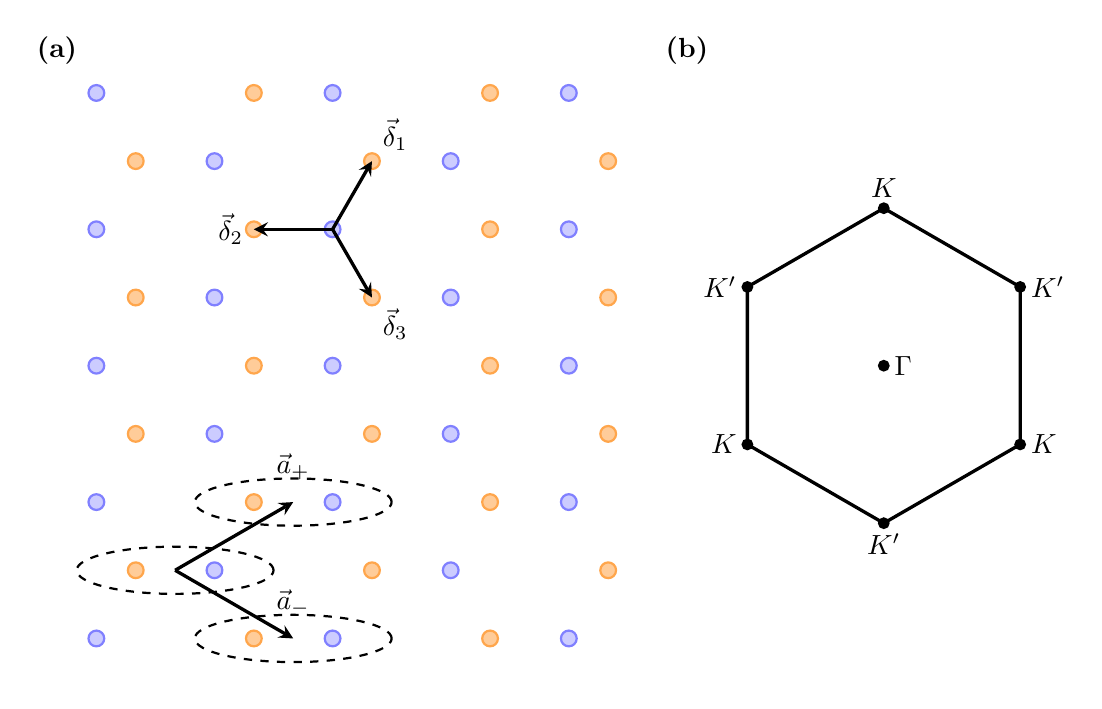
\begin{tikzpicture}															

	% Graphene lattice, sublattices different colors, nearest neighbor vectors and lattice vectors
	\begin{scope}[xshift=-3.5 cm,>=stealth,
		nnarrow/.style={color=black,very thick, ->},					% Nearest neighbor vectors
		A/.style={circle,draw=blue!50,fill=blue!20,
			thick,minimum size=2 mm,inner sep=0pt}, 					% A sublattice dots
		B/.style={circle,draw=orange!70,fill=orange!40,
			thick,minimum size=2mm,inner sep=0pt},						% B sublattice dots
		el1/.style={x radius=1.25*\alat,y radius=.3*\alat},				% Style for the ellipse
		el2/.style={dashed,thick}]										% Style for the ellipse draw

		%This scope is clipped to limit the drawn lattice to a square
		\clip (-3.5cm,-4cm) rectangle(4cm,4cm);
		% Draw the lattice
		\foreach \ip in {-3,-2,...,3}
			\foreach \im in {-3,-2,...,3}
			{
			\node at (\ip*\alat*3/2+\im*\alat*3/2      ,\ip*\sqth*\alat/2-\im*\sqth*\alat/2) [A] {};
			\node at (\ip*\alat*3/2+\im*\alat*3/2-\alat,\ip*\sqth*\alat/2-\im*\sqth*\alat/2) [B] {};
			}

		% Draw the nearest neighbor vectors
		\draw[nnarrow] (0,\alat*\sqth) -- +(60 :\alat) node[anchor=south west]{$\vec{\delta}_1$};
		\draw[nnarrow] (0,\alat*\sqth) -- +(180:\alat) node[anchor=east      ]{$\vec{\delta}_2$};
		\draw[nnarrow] (0,\alat*\sqth) -- +(-60:\alat) node[anchor=north west]{$\vec{\delta}_3$};
		
		% Draw the lattice vectors
		\draw[nnarrow] (240:3*\alat) ++(-\alat/2,0) -- +( 30:\sqth*\alat) node[circle,anchor=south]{$\vec{a}_+$};
		\draw[nnarrow] (240:3*\alat) ++(-\alat/2,0) -- +(-30:\sqth*\alat) node[circle,anchor=south]{$\vec{a}_-$};

		% Ellipses around two atom basis
		\draw[el2] (240:3*\alat) ++(-\alat/2,0) +(  0,0          ) ellipse[el1];
		\draw[el2] (240:3*\alat) ++(-\alat/2,0) +( 30:\sqth*\alat) ellipse[el1];
		\draw[el2] (240:3*\alat) ++(-\alat/2,0) +(-30:\sqth*\alat) ellipse[el1];
	\end{scope}

	% Reciprocal space BZ and high symmetry points
	\begin{scope}[xshift=3.5cm,
		BZ/.style={color=black,fill=black,very thick},
		circ2/.style={radius=1.5pt}]

		% Draw the BZ
		\draw[BZ]
			( 30:\Klen) circle[circ2] node[anchor=west] {$\bm{K'}$} --
			( 90:\Klen) circle[circ2] node[anchor=south]{$\bm{K}$}  --
			(150:\Klen) circle[circ2] node[anchor=east] {$\bm{K'}$} -- 
			(210:\Klen) circle[circ2] node[anchor=east] {$\bm{K}$}  -- 
			(270:\Klen) circle[circ2] node[anchor=north]{$\bm{K'}$} -- 
			(330:\Klen) circle[circ2] node[anchor=west] {$\bm{K}$}  -- 
			( 30:\Klen);

		% Label the high symmetry points
		\draw[BZ] (0,0) circle[circ2] node[anchor=west]{$\Gamma$};
	\end{scope}

	% (a) and (b) labels
	\node at (-7cm,4cm) {\textbf{(a)}};
	\node at ( 1cm,4cm) {\textbf{(b)}};
\end{tikzpicture}
	\end{center}
	\caption{\label{fig:TB:geometry} (a) Real space graphene lattice with the A sub-lattice in orange, the B sub-lattice in blue, nearest neighbor vectors ($\vec \delta_1$, $\vec \delta_2$, and $\vec \delta_3$) shown as arrows, and lattice vectors ($\vec a_+$ and $\vec a_-$) shown translating the two atom basis. (b) First Brillouin zone with the $\Gamma$ point and equivalent $\bm{K}$ and $\bm{K'}$ points indicated.}
\end{figure}

In its unperturbed state, the carbon atoms in the graphene lattice are arrayed in a hexagon as shown in Figure \ref{fig:TB:geometry}(a).
Throughout the x axis will be taken in the graphene arm chair direction as shown.
Since a hexagonal lattice is not a Bravais lattice, the lattice is treated as a triangular Bravais lattice with a two atom bases.
In figure \ref{fig:TB:geometry}(a) the A sub-lattice is colored orange and the B sub-lattice is colored blue.
The lattice is created by arraying the two atoms basic using the lattice vectors $\vec{a}_+=\frac{3}{2} a \hat{x}+\frac{\sqrt{3}}{2} a \hat{y}$ and $\vec{a}_-=\frac{3}{2} a \hat{x}-\frac{\sqrt{3}}{2} a \hat{y}$ where a is the distance between nearest neighbors, $a=1.4 \ l\angstrom$ for graphene.
The three nearest neighbor vectors are given by:
\begin{align*}
	\vec \delta_1&=\frac{a}{2}\hat{x}+\frac{\sqrt{3} a}{2}\hat{y}\\
	\vec \delta_2&=\frac{a}{2}\hat{x}-\frac{\sqrt{3} a}{2}\hat{y}\\
	\vec \delta_3&=-a \hat{x}
\end{align*}

The Brillouin zone of graphene is shown in Figure \ref{fig:TB:geometry}(b).
Like the graphene lattice the Brillouin zone is hexagonal, however it is rotated 30 degrees relative to the crystal axis.
The $\Gamma$ point is at the center of the Brillouin zone while the $\bm{K}$ and $\bm{K'}$ are at the corners.
It should be noted that only 2 of the 6 corners of the hexagon are unique, the others can be connected by reciprocal lattice vectors.
The position of the $\bm{K}$ and $\bm{K'}$ points are given by:
\begin{align*}
	\bm{K}&=-\bm{K'}=\frac{4 \pi}{3 \sqrt{3} a} \hat{y} \\
	\bm{K}&=-\bm{K'}= \frac{2 \pi}{3 a} \hat{x}-\frac{2 \pi}{3 \sqrt{3} a} \hat{y} \\
	\bm{K}&=-\bm{K'}=-\frac{2 \pi}{3 a} \hat{x}-\frac{2 \pi}{3 \sqrt{3} a} \hat{y}
\end{align*}
with the first pair the easiest to work with.

In later sections this discussion will be expanded to take into account strain and phonons perturbing the graphene lattice.
In both cases the changes in graphene's electronic dispersion originates from changes in the position of the atoms.

\section{Electronic dispersion}
Since the tight binding formalism is used universally in this work, this section will start with a brief motivation of its form.
Afterward, the nearest neighbor tight binding formalism will be applied to graphene.

In second quantization, the total energy in the system is written as:
\begin{equation*}
	H=\sum_{\vec{k},\sigma} c^{\dagger}_{\vec{k},\sigma} c__{\vec{k},\sigma} \epsilon_{\vec{k}}
\end{equation*}
where $c^{\dagger}_{\vec{k},\sigma}$ and $c_{\vec{k},\sigma}$ are the creation and annihilation operators for an electrons with wave-vector $\vec{k}$ and spin $\sigma$ and $\epsilon_{\vec{k}}$ is the energy of the electron with wave-vector $\vec{k}$.
The product $c^{\dagger}_{\vec{k},\sigma} c__{\vec{k},\sigma}$ is then a number operator.
This is a very natural definition of the energy; the equation simply sums the energy one wave-vector at a time.

% Here justification of this approximation--applicable when atoms aren't too close...
\begin{align*}
	c^{\dagger}_{\vec{k},\sigma}&=\frac{1}{\sqrt{N}}\sum_{\vec{R}_i} e^{ i \vec{k} \cdot \vec{R}_i} c_{i,\sigma} \\
	c          _{\vec{k},\sigma}&=\frac{1}{\sqrt{N}}\sum_{\vec{R}_i} e^{-i \vec{k} \cdot \vec{R}_i} c_{i,\sigma} \\
\end{align*}
The Hamiltonian becomes:
\begin{align*}
	H&=-\sum_{\vec{R}_i, \vec{R}_j,\sigma} (-) \sum_{\vec{k}}\frac{1}{N} e^{i \vec{k} \cdot (\vec{R}_i-\vec{R}_j)}
	 \epsilon_{\vec{k}} c^{\dagger}_{i,\sigma} c__{j,\sigma} \\
	 &=-\sum_{<i,j>,\sigma} t_{i,j} c^{\dagger}_{i,\sigma} c__{j,\sigma} + \text{H.C},\\
\end{align*}
where the final sum is over $<i,j>$ nearest neighbor pairs and $t_{i,j}=-\sum_{\vec{k}}\frac{1}{N} e^{i \vec{k} \cdot (\vec{R}_i-\vec{R}_j)}\epsilon_{\vec{k}}$ is the hopping energy.
This seemingly complicated parameter has an easy interpretation when the final form of the Hamiltonian is considered.
The hopping energy is the energy associated with removing an electron from atom $j$ and putting it on atom $i$.
As will be illustrate for graphene, this tight binding formalism provides a simple but powerful method of calculating band structures.

The physics relevant for this work is captured by the nearest neighbor tight binding model, the lowest order tight binding approximation.
For graphene, when an electron hops between nearest neighbor, it changes sub-lattice.
The nearest neighbor Hamiltonian reflects this:
\begin{equation*}
	H=-t \sum_{<i,j>} (a_i^{\dagger} b_j + \text{H.C.}),
\end{equation*}
where the hopping energy $t$ gives the energy it takes to remove an electron from the jth atom in the B sub-lattice with the B sub-lattice annihilation operator $b_j$ and put an electron on it nearest neighbor, the ith atom in the A sub-lattice, using the A sub-lattice creation operator $a_i$.
The sum is restricted to $<i,j>$ nearest neighbor pairs.
Finally the Hermitian conjugate, $\text{H.C.}$, accounts for the hopping from the A sub-lattice to the B sub-lattice and also ensures that the Hamiltonian is Hermitian.

The Hamiltonian is simplified by writing the creation and annihilation operators in Fourier space.
There is some freedom in choosing the phase factors.
They can either be chosen so that the operators are expanded around the position of each atom or instead they can be expanded around the position of the atomic basis occupied by the atom.
Both approaches yield the same result if one is consistent\cite{Bena2009}.
Here the operators are expanded about the atomic basis.
This will make the correspondence with the Dirac-Weyl equation more clear.
\begin{align*}
	a_i^{\dagger}&=\frac{1}{\sqrt{N}}\sum_{\vec{k} } e^{ i \vec{k}  \cdot \vec{R}_i} a_{\vec{k} }^{\dagger} \\
	b_j          &=\frac{1}{\sqrt{N}}\sum_{\vec{k}'} e^{-i \vec{k}' \cdot \vec{R}_j} b_{\vec{k}'} \\
\end{align*}
where $R_i$ and $R_j$ are the position of the $ith$ and $jth$ atomic basis respectfully.  The Hamiltonian becomes:
\begin{align}
	H&=-t \frac{1}{N} \sum{<i,j>}\sum_{\vec{k},\vec{k'}}(e^{i \vec{k}}+\text{H.C.})\\
	& \label{eq:TB:RealSpace}
\end{align}

\section{Dirac-Weyl electrons}